\documentclass{beamer}
\usetheme{Warsaw}

\usepackage[utf8]{inputenc}
\usepackage{fancybox}
\usepackage{multimedia} 
\usepackage{subfig}
\usepackage{amsmath}
\usepackage{hyperref}
\hypersetup{
    colorlinks=true,     
    urlcolor=blue
}
\usepackage[all]{xy}

\setbeamertemplate{footline}[frame number]


\begin{document}


\title[Stochastik] % (optional, only for long titles)
{Wahrscheinlichkeitstheorie und Statistik (Stochastik)
\\
\includegraphics[scale=0.5]{img/craps}
}
\subtitle{}
\author[Dr. Johannes Riesterer] % (optional, for multiple authors)
{Dr.  rer. nat. Johannes Riesterer}

\date[KPT 2004] % (optional)
{}

\subject{Stochastik}

\frame{\titlepage}

\begin{frame}
    \frametitle{Wesentliche Begriffe}
\framesubtitle{}

\begin{figure}[htp]
      \centering
    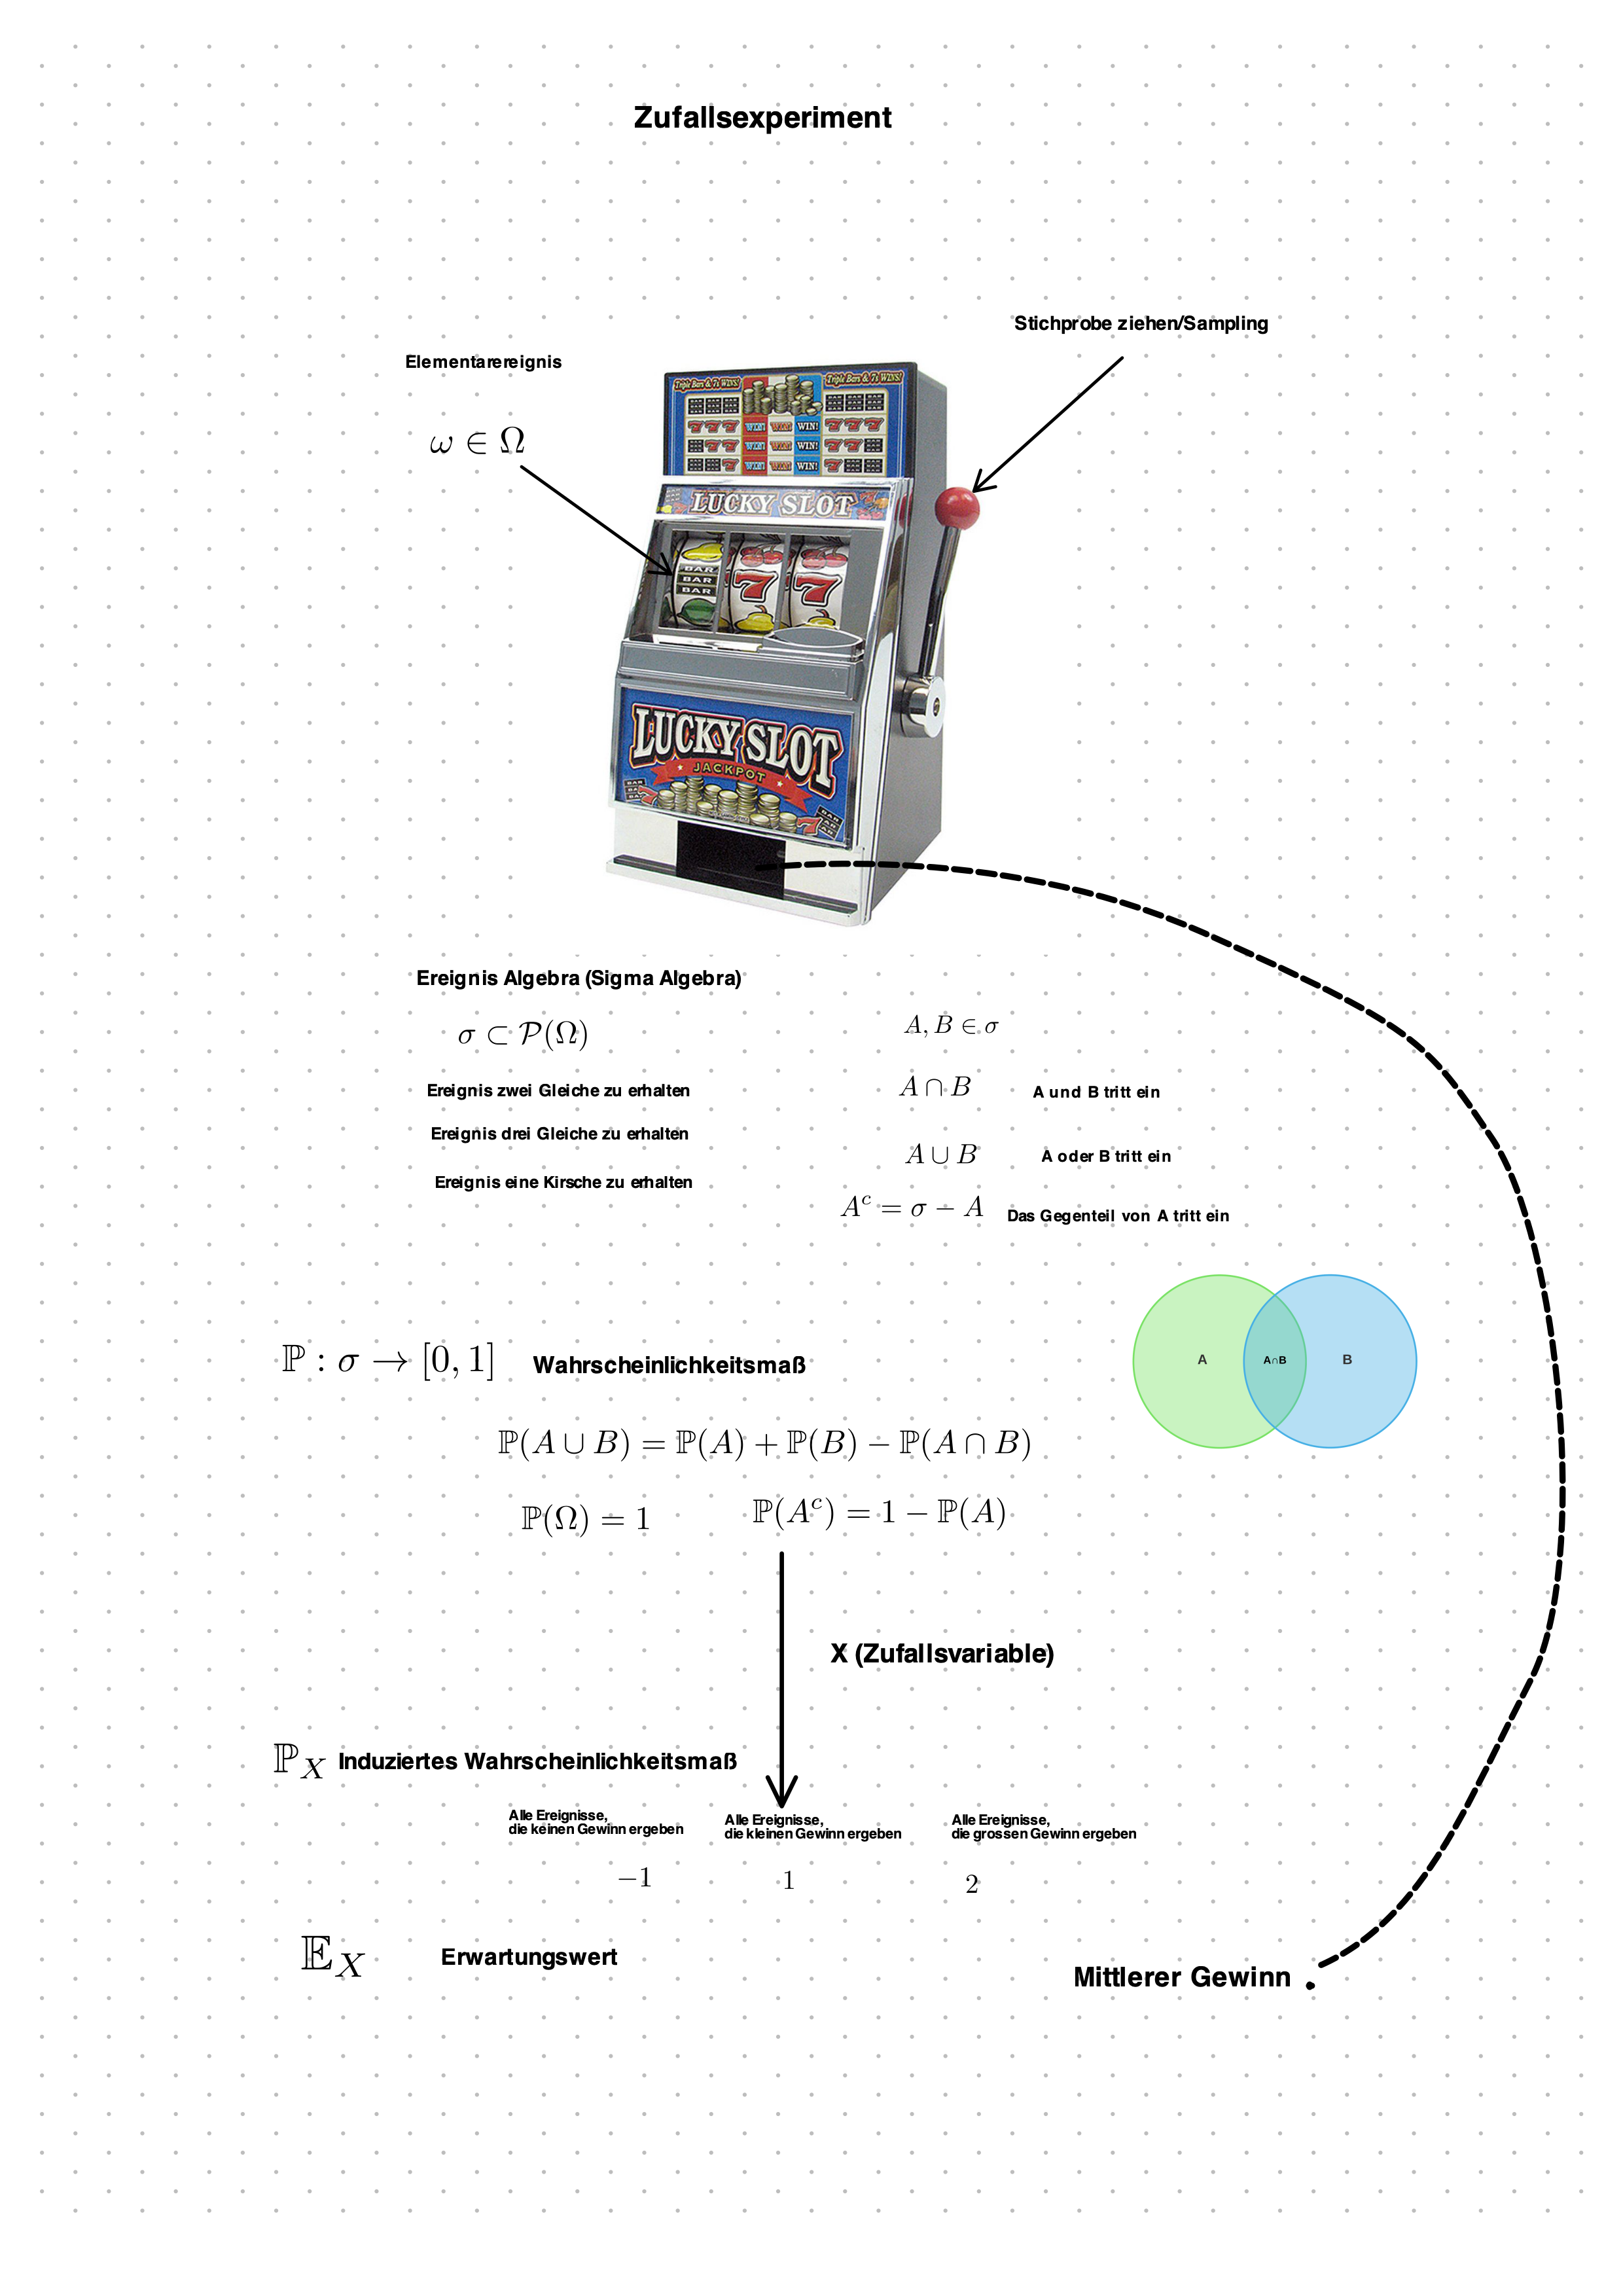
\includegraphics[width=0.5\textwidth]{img/overview_prob.png}
\end{figure}

 \end{frame}


\end{document}
